%!TEX encoding = UTF-8


\documentclass[UTF8]{ctexart}

\usepackage{tikz}
\usepackage{amssymb}
\usepackage{amsmath}

\usetikzlibrary{calc}
\usepackage{fontspec}

% Set up a font that supports Chinese characters
% \setmainfont{SimSun}[Path=./] % Specify the path if the font is not in the system fonts
% Alternatively, you can use other fonts like:
% \setmainfont{Microsoft YaHei}
% \setmainfont{NotoSansCJKsc-Regular.otf}


\setmainfont{Noto Sans CJK SC}


\begin{document}

△DEF 为正三角形 AD=BE=CF

求证 △ABC为正三角形


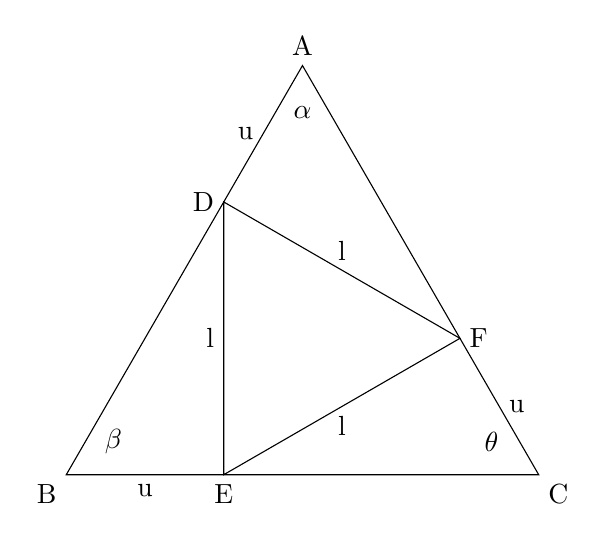
\begin{tikzpicture}[scale=6]
    % Define coordinates for the outer equilateral triangle
    \coordinate (A) at (0, {sqrt(3)/2});
    \coordinate (B) at (-0.5, 0);
    \coordinate (C) at (0.5, 0);
    
    % Define D relative to A (1/3 of the way down from A)
    \coordinate (D) at ($(A)!1/3!(B)$);
    \coordinate (E) at ($(B)!1/3!(C)$);
    \coordinate (F) at ($(C)!1/3!(A)$);
    
    % Draw the main triangle
    \draw (A) -- (B) -- (C) -- cycle;
    
    % Draw internal lines
    \draw (D) -- (E) -- (F) -- cycle;
    
    % Label points
    \node[above]        at (A) {A};
    \node[below left]   at (B) {B};
    \node[below right]  at (C) {C};
    \node[left]         at (D) {D};
    \node[below]        at (E) {E};
    \node[right]        at (F) {F};

    \node at ($(A) + (0, -0.1)$) {$\alpha$};
    \node at ($(B) + (0.1, 0.07)$) {$\beta$};    
    \node at ($(C) + (-0.1, 0.07)$) {$\theta$};


    % length `u`
    \node at ($(A)!0.5!(D)$) [left] {u};
    \node at ($(B)!0.5!(E)$) [below] {u};
    \node at ($(C)!0.5!(F)$) [right] {u};

	% length `l`
    \node at ($(D)!0.5!(E)$) [left] {l};
    \node at ($(E)!0.5!(F)$) [below] {l};
    \node at ($(F)!0.5!(D)$) [above] {l};
    
\end{tikzpicture}





假设 
$\angle \alpha < \angle \theta$


\begin{align}

\angle \alpha > \angle \theta

\because \cos \alpha = \frac{u^2 + |AF|^2 - l^2}{2 u |AF|} = \frac{u^2 + x^2 - l^2}{2 u x}

\therefore (\cos \alpha)' &= (\frac{(u^2 - l^2)}{2u} \frac{1}{x} + \frac{x}{2u})'
                          &= \frac{(l^2 - u^2)}{2u} \frac{1}{x^2} + \frac{1}{2u}
                          
                          

\end{align}

如果 $l > u$, 随着 $\alpha$ 增大 $|AF|$ 减小

\begin{align}

\angle \alpha < \angle \theta

=> |AF| < |CE|

=> |AC| < |BC|

=> \angle \beta < \angle \alpha

=> |BD| > |AF|

=> |AB| > |AC|

=> \angle \theta > \angle \beta

=> |CE| < |BD|

=> |BC| < |AB|

=> \angle \alpha > \angle \theta

\end{align}
	
\end{document}
